
%
%
\subsection{JCore}
The JCore contains several main components of our engine. Those contain the evaluation of the database and the enablement of activities in the ExecutionService etc.\\
In the JCore reside some of the most fundamental funtionalities that our engine offers. They include the possibility to run activities sequentially. Supported activity-types are user-task and email-task.\\
With PCM activities can be enabled from controllflow or dataflow point of view. That is the reason why we support dataobjects and their state transitions. Further activities can be referenced in PCM, which has the effect during execution, that referenced activities, which are enabled and share the same set of pre- and postconditions, can both switch to the state 'running' if one of them is being activated.\\
Also PCM-fragments consist of a subset of BPMN. Currently we support start- and end-events, activities and XOR- and AND-Gateways.


\subsubsection{Class diagram}

The ExecutionService is the class that manages the complete JCore. The ExecutionService manages all ScenarioInstances and provides methods to interact with a scenario instance, for example to do an activity.\\
The ScenarioInstance represents an instance of a PCM scenario. It saves all FragmentInstances, ControlNodeInstances and DataObjectInstances. If a ScenarioInstance get initialized it initializes all FragmentInstances and DataObjectInstances.\\
The DataObjectInstances represent PCM data objects. They have a state and list of all there DataAttributeInstances. The DataAttributeInstance represent the data attributes and save the value and the type of the attribute.\\
The FragmentInstances have one function they initialize all ControlNodeInstances.
ControlNodeInstances are ActivityInstances and GatewayInstances which are shown in the PCM model. All ControlNodeInstances have a StateMachine,  a IncomingBehavior and a OutgoingBehavior. The StateMachine controls the state of the ControlNodeInstance and does the state transitions. The IncomingBehavior controls the incoming control flow. This is important for PCM gateways, because this behavior decides if a AND gateway for example can be activated. The OutgoingBehavior controls the outgoing control flow. For Example the data object output states for an activity are set here.\\
An ActivityInstance also have an TaskExecutionBehavior this behavior manages all things that happens if you execute the activity. This can be the HumanTaskExecutionBehavior that sets the data attribute states or a service task execution behavior like the EmailTaskExecutionBehavior that send automatic an eMail.\\

\begin{figure}[h!]
\centering
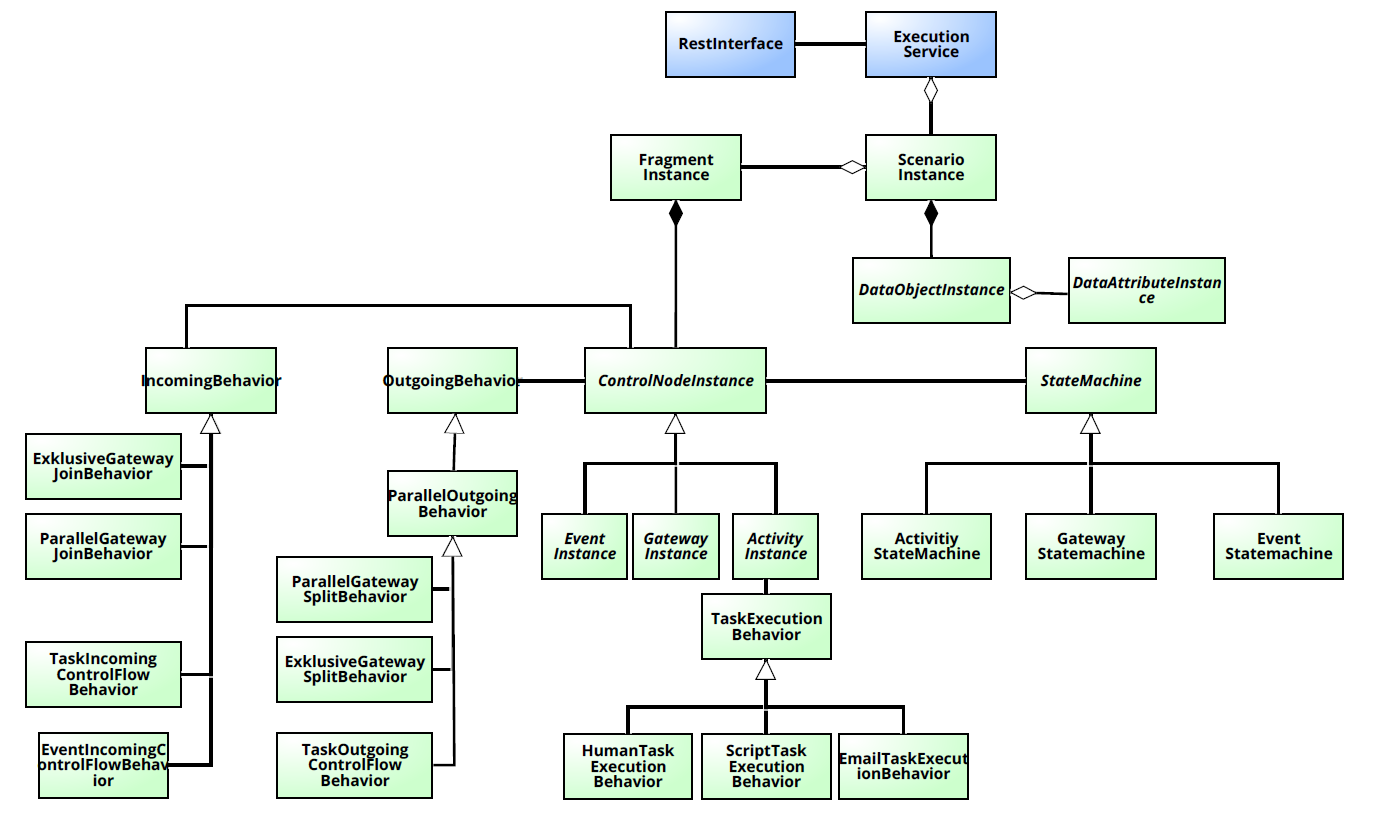
\includegraphics[width=6in]{img/ClassDiagramm.png}
\caption{userview}
\label{fig:userview}
\end{figure}

\subsubsection{E-Mail-Tasks}
\label{jCore:MailTask}
The JEngine supports the execution of E-MailTasks. All of the E-Mail configurations are saved in the database in table \textit{emailconfiguration}. Every E-Mail-Task which is modeled as described in section \ref{pe:email} gets its own database entry whith the corresponding controlnodeID (that's the databaseID, not the modelID from the XML) of the Mail Task.\\
The default template holds the databaseID -1. The values of the attributes from the default template are copied for each individual E-Mail-Task. In so far, the receivermailaddress, sendmailaddress, subject and messagecontent from the default template are used, if not specified differently. The databaseID and the controlnodeID are set automatically. If you wish to make an own configuration for the Mail Task, you can use the frontEnd 
\begin{math}(Admin\rightarrow Mail Config)\end{math}
by selecting the scenario, choosing the Activity and clicking on \textit{Show Details}. After a window with the default content opens, you can enter the receiver, subject, and message. Otherwise you can also change the values in the database.\\
\textbf{Attributes.} It is possible to access the values of dataAttributes in the message content, subject or e-Mail address by typing the following expression:
\begin{align}
\textbf{\#dataobjectName.dataobjectAttributeName} \nonumber
\end{align}
This expression gets replaced by the value of \textit{dataobjectAttributeName} which is an attribute of \textit{dataobjectName}.

\subsubsection{WebServiceTasks}
The JEngine supports the execution of WebServiceTasks. All of the WebService configurations are saved in the database in tables \textit{webservicetasklink, webservicetaskpost, webservicetaskattribute}. Initial Webservice Tasks have no configuration entries in the database. The user have to configure the Tasks.\\
In the database table \textit{webservicelink} is the method of the request defined. This can be \textit{GET, PUT or POST}.\\
In the database table \textit{webservicepost} gets the JSON for the PUT/POST request saved. The information from the dataobject and dataattributes can be used in the request. To access the values and states you have to type following expression:
\textbf{\#dataobjectName.dataobjectAttributeName} \nonumber for the attribute value or
\textbf{\#dataobjectName} \nonumber for the dataobject state.\\
In the database table \textit{webserviceattribute} is defined which values from the JSON are saved in which dataattribute. The Engine uses the \textit{key} to know how to access the JSON. The \textit{order} ist the order in which the \textit{keys} are used.
%
%

\subsubsection{XOR Gateways}

The JCore can execute XOR Gateways. The syntax of the conditions is shown by the following grammar. Expressions like \textit{#Dataobject.Dataattribute} or \textit{#Dataobject} are replaced with Dataattribute values and Dataobject states.\\
\begin{lstlisting}

expression  ::=     expr2 (OPERATOR expr2)*;
expr2       ::=     NAME COMPARISON NAME;
NAME        ::=     CHARAC | CHARAC  DOT CHARAC;
CHARAC      ::=     [#]('A'..'Z' | 'a'..'z' | '0'..'9')+;
COMPARISON  ::=     '=' | '<' | '>' | '<=' | '>=';
DOT         ::=     '.';
OPERATOR    ::=     ' & ' | ' | ' | '&' | '|';

\end{lstlisting}

\subsubsection{REST-API}

veraltet

\iffalse
Um eine Kommunikation zwischen unseren verschieden Elementen der Engine und des Front-Ends zu ermöglichen, haben wir uns für ein REST-Interface entschieden. Dabei unterstützen wir bisher 2 Methoden: GET und POST.
\begin{enumerate}
%hier beginnt Aufzählung unserer REST Methoden
\item \textbf{@GET:}\\
Die GET-Requests existieren, um den Nutzern der Engine über ein User Interface eine Möglichkeit zu bieten, einzusehen welche Aktivitäten noch zu bearbeiten sind (also offen sind) bzw. welche Aktivitäten zu welcher Scenarioinstanz gehören und ähnliches. \\

1.1.\\ Um offene bzw. geschlossene Aktivitäten einer ScenarioInstanz ausgegeben zu bekommen, muss ein GET mit folgender URL ausgeführt werden:\\
\textbf{\textit{http://172.16.64.113:8080/JEngine/Scenario/\\\{ScenarioID\}/\{ScenarioInstanceID\}/\{Status\}}}\\

\textbf{Variablen die benutzt werden:}\\
\textit{ScenarioID:} hier wird die ID des Scenarios erwartet. Dabei handelt es sich um einen Integer-Wert.\\
\textit{ScenarioInstanceID:} hier wird die ID der ScenarioInstanz erwartet. Dabei handelt es sich um einen Integer-Wert.\\
\textit{Status:} Der Status ist vom Typ String und muss ein Element der Menge\textbf{\textit{\{terminated, enabled\}}} sein.\\

\textbf{Dabei können folgende Fehler geworfen werden:}\\
\textit{Error: not a correct scenario instance}\\ Dies bedeutet das eine ScenarioInstanzID angegeben worden ist, die nicht existiert.\\
\textit{Error: status not clear}\\ Dieser Fehler besagt, dass ein Status angegeben wurde, der nicht der Menge \textbf{\textit{\{terminated, enabled\}}} entspricht.\\

1.2. \\Wenn man wissen möchte, welche Szenarien man in der JEngine starten kann, erhält man diese über folgende GET URL:\\
\textbf{\textit{http://172.16.64.113:8080/JEngine/Scenario/\\Show}}\\

1.3.\\ Um alle ScenarioInstanzen eines Szenarios zu bekommen, muss ein GET-Request mit folgender URL ausgeführt werden:\\
\textbf{\textit{http://172.16.64.113:8080/JEngine/Scenario/\\Instances/\{ScenarioID\}}}\\

\textbf{Variable die benutzt wird:}\\
\textit{ScenarioID:} Dabei handelt es sich um einen Integer, der die ID des zu betrachtenden Szenarios angibt.\\

\textbf{Dabei kann folgender Fehler geworfen werden:}\\
\textit{Error: not a correct scenario}\\ Dieser tritt auf, wenn eine ID übergeben wurde, die nicht existiert.\\

1.4.\\ Wenn man alle Datenobjekte in ihren entsprechenden Zuständen anzeigen möchte, bezogen auf eine ScenarioInstanz, muss ein GET-Request mit folgender URL ausgfeührt werden:\\
\textbf{\textit{http://172.16.64.113:8080/JEngine/Scenario/\\DataObjects/\{ScenarioID\}/\{ScenarioInstanceID\}}}\\

\textbf{Variablen die benutzt werden:}\\
\textit{ScenarioID:} hier wird die ID des Scenarios erwartet. Dabei handelt es sich um einen Integer-Wert.\\
\textit{ScenarioInstanceID:} hier wird die ID der ScenarioInstanz erwartet. Dabei handelt es sich um einen Integer-Wert.\\

\textbf{Dabei kann folgender Fehler geworfen werden:}\\
\textit{Error: not a correct scenario instance}\\ Wenn eine falsche ScenarioInstanzID angegeben wird, produziert es diesen Fehler.\\

1.5.\\ Um von einer SzenrioInstanzID die dazugehörige ScenrioID zu erhalten, kann ein GET-Request mit folgender URL ausgeführt werden:\\ 
\textbf{\textit{http://172.16.64.113:8080/JEngine/Scenario/\\Get/ScenarioID/\{ScenarioInstanceID\}}}\\

\textbf{Variable die benutzt wird:}\\
\textit{ScenarioInstanceID:} hier wird die ID der ScenarioInstanz erwartet. Dabei handelt es sich um einen Integer-Wert.\\

\textbf{Dabei kann folgender Fehler geworfen werden:}\\
\textit{Error: not a correct scenario instance} \\ Wurde eine ScenarioInstanzID angegeben, die nicht existiert, wird dieser Fehler geworfen.\\

1.6.\\ Wenn man eine AktivitätsInstanzId besitzt, und das dazugehörige Label wissen möchte, kann man einen GET-Request mit folgender URL ausführen:\\
\textit{\textbf{http://172.16.64.113:8080/JEngine/Scenario/\\ActivityID/\{Activity\}}}

\textbf{Variable die benutzt wird:}\\
\textit{Activity:} hier wird die ID der AktivitätsInstanz erwartet. Dabei handelt es sich um einen Integer-Wert.\\

\textbf{Dabei kann folgender Fehler geworfen werden:}\\
\textit{Error: not correct Activity ID}\\ Wurde eine AktivitätsInstanzID angegeben, die nicht existiert, wird dieser Fehler geworfen.\\

\item \textbf{@POST:}\\
Über POST-Request ist es möglich, Aktivitäten zu starten sowie gestartete Aktivitäten zu terminieren. Außerdem besteht auch die Möglichkeit ganze Szenarien zu starten, falls dies benötigt wird. All dies soll mit der Funktion ausgestattet sein, dass man dazu noch einen Kommentar abgeben kann.\\

2.1.\\ Um über einen POST-Request Aktivitäten zu starten bzw. zu beenden, wird die folgende URL genutzt:\\
\textit{\textbf{http://172.16.64.113:8080/JEngine/Scenario/\\\{ScenarioID\}/\{ScenarioInstanceID\}/\\\{ActivityID\}/\{Status\}/comment}}\\

\textbf{Variablen die benutzt werden:}\\
\textit{ScenarioID:} hier wird die ID des Scenarios erwartet. Dabei handelt es sich um einen Integer-Wert.\\
\textit{ScenarioInstanceID:} hier wird die ID der ScenarioInstanz erwartet. Dabei handelt es sich um einen Integer-Wert.\\
\textit{ActivityID:} hier wird die ID der AktivitätsInstanz erwartet. Dabei handelt es sich um einen Integer-Wert.\\
\textit{Status:} Der Status ist vom Typ String und muss ein Element der Menge\textbf{\textit{\{terminate, begin\}}} sein.\\

\textbf{Im Fehlerfall:}\\
Wird versucht eine Aktivität zu starten, die nicht existiert bzw. eine Aktivität zu beenden, die gar nicht gestartet war, wird einem ein Boolean mit dem Wert \textit{false} zurückgegeben.\\

2.2.\\ Wenn eine neue Instanz eines Szenarios gestartet werden soll, nutzt man den POST-Request mit folgender URL:\\
\textit{\textbf{http://172.16.64.113:8080/JEngine/Scenario/\\Start/\{ScenarioID\}}}\\

\textbf{Variable die benutzt wird:}\\
\textit{ScenarioID:} hier wird die ID des Scenarios erwartet. Dabei handelt es sich um einen Integer-Wert.\\

\textbf{Im Fehlerfall:}\\
Wird versucht ein Szenario zu starten, das nicht existiert, wird einem ein Integer mit dem Wert \textit{-1} zurückgegeben.\\

\end{enumerate}


Default URL:
http://172.16.64.113:8080/JEngine/interface/\{version\}/\{language\}/?

as parameter:
scenario
returns all scenarios
 
scenario=1
returns all instances

scenario=1\& runtime
returns all instances with runtime

instanceid=1\& status=enabled
returns all enabled activities

activityid=2
returns all information for this activity

users
returns all users

roles
roles returns all roles


timestamp ISO-8601
\fi

for more informations about the REST please have a look at the REST Specification:
https://github.com/BP2014W1/JEngine/blob/dev/docu/JEngine_REST_Specs.pdf


%
%
\subsubsection{ExecutionService}
The ExecutionService is the component that is being used by the REST-API. So this component of the JEngine is essential to process queries that have been received via the REST interface. It establishes a database-connection to run queries on it. Most queries require the ID of an object to gather more information. Additionaly there are methods to instantiate activities and whole scenarios respectively.